%\documentclass[final]{article}
\documentclass[]{article}
\usepackage{geometry}
\geometry{
	a4paper,
	total={170mm,257mm},
	left=0.75in,
	top=0.75in,
	right=0.75in,
	bottom=1in,
}
\newcommand{\extramargin}[1]{}
%\newcommand{\extramargin}[1]{
	%	\setlength{\paperwidth}{250mm}
	%	\setlength{\evensidemargin}{-15mm}
	%	\setlength{\oddsidemargin}{-15mm}
	%}
\usepackage{gensymb}
\usepackage{lipsum}
\usepackage{graphicx}
\usepackage{epstopdf, epsfig}
\usepackage{amsmath}
\usepackage[url=false,
backend=bibtex,
style=authoryear-comp,
giveninits=true,
doi=true,
isbn=true,
backref=false,
dashed=false,
maxcitenames=2,
maxbibnames=99,
natbib=true]{biblatex}
\DeclareNameAlias{author}{last-first}
\DeclareFieldFormat
[article,inbook,incollection,inproceedings,patent,thesis,
unpublished,techreport,misc,book]
{title}{#1}
\renewcommand*{\revsdnamepunct}{}
\renewbibmacro{in:}{}
\usepackage{xpatch}
\xpatchbibmacro{date+extradate}{%
	\printtext[parens]%
}{%
	\setunit*{\space}%
	\printtext%
}{}{} 


\addbibresource{../Main/ViscousDropImpact_v2.bib}
\nonfrenchspacing
\setlength\parindent{0pt}
\usepackage{siunitx}
\usepackage{xcolor}
\usepackage{mathrsfs}
\usepackage[colorlinks,citecolor=purple,urlcolor=blue]{hyperref}
\newcommand*\blue{\textcolor{blue}}
\newcommand*\red{\textcolor{red}}
\newcommand{\VS}[1]{{\textcolor{orange}{#1}}}

\newcommand{\oo}{\color{magenta} \normalfont}
\newcommand{\bb}{\color{black} \normalfont}

\newcommand{\vs}{\color{orange} \normalfont}

\renewcommand{\thefigure}{R\arabic{figure}}

\usepackage[obeyFinal,colorinlistoftodos, textwidth=60mm, shadow]{todonotes}
% todonotes specific macros begin!
\newcommand{\todoInsertref}[2]{\todo[color=green!40, #1]{#2}}
\newcommand{\todoExplaininDetails}[2]{\todo[color=orange!40, #1]{#2}}
\newcommand{\todoUrgent}[2]{\todo[color=red!40, #1]{#2}}
\newcommand{\todoSansUrgent}[2]{\todo[color=yellow!40, #1]{#2}}
\extramargin
%% todonotes specific macros end!

%opening
\title{Reply to Referee 2}
\author{Vatsal Sanjay, Bin Zhang, Cunjing Lv, and Detlef Lohse}
\date{}
\begin{document}
	
\maketitle
	
\textit{The authors have made some improvements to the manuscript based on the feedback provided, however some concerns were not fully addressed, as described below. I will use the same number scheme as in the prior report for consistency. I am content with the response for points that are not re-addressed below.}

We thank the referee for carefully reading our manuscript and providing valuable feedback and suggestions. We have reviewed the referee's comments and made changes based on their suggestions. Below, we offer a point-to-point reply to each of the referee's comments and include the changes made in the manuscript. The referee's comments are in italics, and our replies are in plain black. Changes in the manuscript are highlighted in magenta.


\begin{enumerate}
	\item[$\bullet$] \textit{While I appreciate the inclusion of two additional force datasets, no new droplet shape profiles were included. For a paper that has a significant experimental component, I am surprised with the lack of direct visualization of the droplet dynamics. At minimum, I would recommend adding droplet shape profile comparisons for the two new data sets. Furthermore, these visualizations (including the one already included) should include a scale bar. Additionally, I would suggest including some experimental videos as supplementary materials.}\\[1mm]
	
	We have modified figure~2 of the main text (see figure~\ref{fig:summary}) to include direct visualization of the droplet dynamics. We have also added three supplementary videos: SM1-SM3. 
	
	\begin{figure}
		\centering
		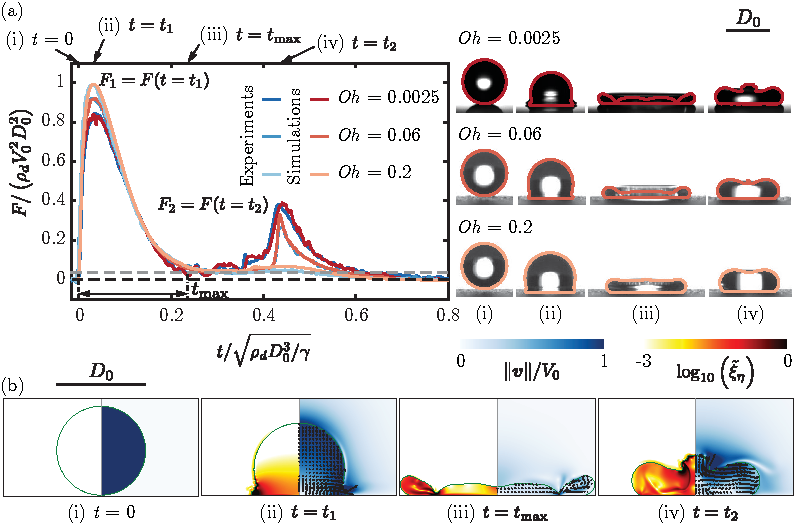
\includegraphics[width=\textwidth]{../Main/Figures/Figure1_summary_v6.pdf}
		\caption{{\oo Comparison of the drop impact force $F(t)$ obtained from experiments and simulations for the three typical cases with impact velocity $V_0 = 1.2\,\si{\meter}/\si{\second}, 0.97\,\si{\meter}/\si{\second}, 0.96\,\si{\meter}/\si{\second}$, diameter $D_0 = 2.05\,\si{\milli\meter}, 2.52\,\si{\milli\meter}, 2.54\,\si{\milli\meter}$, surface tension $\gamma = 72\,\si{\milli\newton}/\si{\meter}, 61\,\si{\milli\newton}/\si{\meter}, 61\,\si{\milli\newton}/\si{\meter}$ and viscosity $\eta_d = 1\,\si{\milli\pascal\second}, 25.3\,\si{\milli\pascal\second}, 80.2\,\si{\milli\pascal\second}$. These parameter give $Oh = 0.0025, 0.06, 0.2$ and $We = 40$.
		For the three cases, the two peak amplitudes, $F_1/(\rho_dV_0^2D_0^2) \approx$ 0.82, 0.92, 0.99 at $t_1 \approx 0.03\sqrt{\rho_dD_0^3/\gamma}$ and $F_2/(\rho_dV_0^2D_0^2) \approx$ 0.37, 0.337, 0.1 at $t_2 \approx 0.42\sqrt{\rho_dD_0^3/\gamma}$, characterize the inertial shock from impact and the Worthington jet before takeoff, respectively. 
		The drop reaches the maximum spreading at $t_{\text{max}}$ when it momentarily stops and retracts until $0.8\sqrt{\rho_dD_0^3/\gamma}$ when the drop takes off ($F = 0$). The black and gray dashed lines in panel (a) mark $F = 0$ and the resolution $F = 0.5\,\si{\milli\newton}$ of our piezoelectric force transducer, respectively.
		(b) Four instances are further elaborated through numerical simulations for ($We = 40, Oh = 0.0025$), namely (i) $t = 0$ (touch-down), (ii) $t = 0.03\sqrt{\rho_dD_0^3/\gamma}$ ($t_1$), (iii) $t = 0.2\sqrt{\rho_dD_0^3/\gamma}$ ($t_{\text{max}}$), and (iv) $t = 0.42\sqrt{\rho_dD_0^3/\gamma}$ ($t_2$).
		The insets of panel (a) exemplify these four instances for the three representative cases illustrated here. The experimental snapshots are overlaid with the drop boundaries from simulations. 
		We stress the excellent agreement between experiments and simulations without any free parameters.
		The left part of each numerical snapshot shows (on a $\log_{10}$ scale) the dimensionless local viscous dissipation function $\tilde{\xi}_\eta \equiv \xi_\eta D_0/\left(\rho_dV_0^3\right) = 2Oh\left(\boldsymbol{\tilde{\mathcal{D}}:\tilde{\mathcal{D}}}\right)$, where $\boldsymbol{\mathcal{D}}$ is the symmetric part of the velocity gradient tensor, and the right part the velocity field magnitude normalized with the impact velocity. The black velocity vectors are plotted in the center of mass reference frame of the drop to clearly elucidate the internal flow.  Also see supplementary videos SM1-SM3.\bb}}
		\label{fig:summary}
	\end{figure}
	
	
	
	\item[$\bullet$] \textit{2. I appreciate the clarification regarding the error bars. However, a proper characterization (and description of the procedure by which they are determined) of the estimated parametric errors is still incomplete. Rather than including additional discussion, the authors reference the supplementary materials of a prior work (Zhang et al. (2022)). In reviewing this work, I cannot identify error assessments on key parameters (such as impact velocity). An error is now included on the droplet size, but there is no discussion of how drop size is determined nor how this error determined. Additionally, the related point regarding horizontal error bars was not addressed. Given that there is no length limit, I would suggest the authors include all details in the present manuscript rather than referring to incomplete discussions in prior work. (Also a minor point: the new horizontal line associated with the force sensor resolution should be described in the caption.)}\\[1mm]
	
	We appreciate the reviewer's insistence on a comprehensive error characterization. We have addressed this concern by adding a new appendix to the manuscript, titled ``Note on the error characterization for the control parameters". We have also modified the caption of figure~2 of the main text to describe the horizontal dashed lines (see figure~\ref{fig:summary}).  
	
	\S~\red{2.1:}\\
	\oo
	Throughout the manuscript, the error bars are of statistical nature (one standard deviation) and originate from repeated trials. They are visible if they are larger than the marker size.  We refer the readers to the supplementary material of \citet{zhang2022impact}  and appendix~A for further details of the experimental setup and error characterization of the dimensionless control parameters.
	
	\section*{Appendix A. Note on the error characterization for the control parameters}
	\label{app:error}
	This appendix outlines the methodology for characterizing experimental errors in quantification of the drop's size and impact velocities which is crucial for accurate calculation of dimensionless control parameters, $We$ and $Oh$.
	The drop diameter determination involves multiple steps. First, we measure the total mass ($M_{100}$) of 100 drops using an electric balance. From this mass, using the liquid density and assuming spherical shape, we calculated the drop diameter ($D_0$). 
	We repeated this process five times, yielding $D_{0,1}$ through $D_{0,5}$. The average of these measurements provided the final drop diameter ($D_0$) and its standard error.
	For impact velocity determination, we extracted data from experimental high-speed imagery. By tracking the drop center's position in successive frames prior to substrate contact, and knowing the frame rate, we calculated the impact velocity. We repeated this process for five trials, obtaining $V_{0,1}$ through $V_{0,5}$. The average of these values gave the final impact velocity ($V_0$) and its standard error.
	
	The standard errors for drop diameters do not exceed $0.13\,\si{\milli\meter}$. For instance, drops with Ohnesorge numbers of $0.0025$, $0.0625$, and $0.2$ have diameters of $2.05 \pm 0.13\,\si{\milli\meter}$, $2.52 \pm 0.11\,\si{\milli\meter}$, and $2.54 \pm 0.09\,\si{\milli\meter}$, respectively. 
	The standard errors for impact velocities did not exceed $0.02\,\si{\meter}/\si{\second}$. For the same $Oh$ values, the impact velocities were $1.2 \pm 0.002\,\si{\meter}/\si{\second}$, $0.97 \pm 0.01\,\si{\meter}/\si{\second}$, and $0.96 \pm 0.01\,\si{\meter}/\si{\second}$, respectively.
	The combined errors in $D_0$ and $V_0$ resulted in approximately $\pm 7\%$ error in Weber number $We$ and $\pm 3\%$ error in Ohnesorge number $Oh$. Consequently, the horizontal error bars, which relate to errors in the control parameters, are smaller than the symbol sizes in our figures.
	\bb
	
	\item[$\bullet$] \textit{3.}
	\begin{itemize}
		\renewcommand\labelitemi{--}
		\item \textit{In the experimental methods, the authors now describe that the Bond number is fixed at 1. Given the change in fluid properties between different solutions (with fixed droplet size), this cannot be the case. This needs to be made more precise. Furthermore, in the authors' prior work (Zhang et al. (2022)), it is mentioned that the Bo is fixed at 0.5 in simulation for similar experimental parameters. Why the change?}\\[1mm]
		
		We appreciate the reviewer's comment regarding the Bond number. 
		The reviewer is correct in pointing out the inconsistency, and we apologize for any confusion this may have caused. We would like to clarify and expand on this point:

		\begin{enumerate}
			\item \textbf{Experimental Bond number range:}
			Indeed, given the variation in fluid properties and drop sizes used in our experiments, the Bond number is not strictly fixed at 1, it only is $\mathcal{O}\left(1\right)$.
			\item \textbf{Simulation Bond number:}
			In our simulations, we chose to use a fixed Bond number of 1 as the representative value. This choice was made to simplify the parameter space and focus on the effects of Weber and Ohnesorge numbers. We have added a new appendix (Appendix B) to address this point and demonstrate the validity of this approach. We have also expanded our discussion in Appendix B to justify our approach and discuss its implications.
			\item \textbf{Difference from previous work:}
			The reviewer correctly notes that in our previous work \citep{zhang2022impact}, we used a fixed Bond number of 0.5 in simulations. The change to $Bo = 1$ in the current work was made to better represent the average experimental conditions. However, as our sensitivity analysis shows, this change hardly affects our results.
		\end{enumerate}		
		
		\S~\red{2.2:}\\
		\oo
		Lastly, we keep the Bond number $Bo$ (see~(1.3)) fixed at 1 throughout the manuscript. In our system, the relevance of gravity is characterized by the dimensionless Froude number $Fr = V_0^2/(gD_0) = We/Bo$ which compares inertia with gravity. Throughout this manuscript, $Fr > 1$ and gravity's role is sub-dominant compared to inertia (for detailed discussion, see appendix~B).
		\bb
		
		\begin{figure}
			\centering
			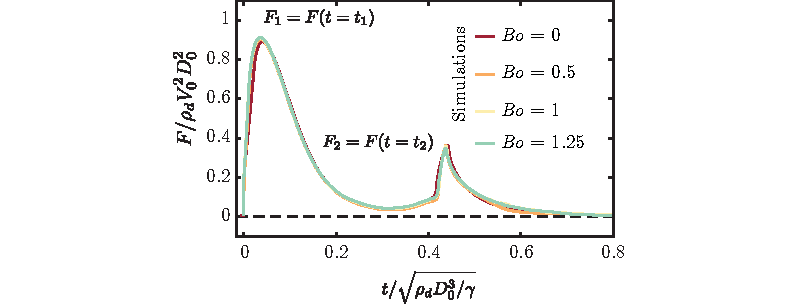
\includegraphics[width=\textwidth]{../main/Figures/figureA1.pdf}
			\caption{{\oo Comparison of the drop impact force $F(t)$ obtained from simulations for the four different Bond numbers $Bo = 0, 0.5, 1, 1.25$. Here, $Oh = 0.06$ and $We = 40$. Both force peaks $F_1$ and $F_2$ as well as time to reach these peaks $t_1$ and $t_2$ are invariant to variation in $Bo$. \bb}}
			\label{fig:AppGravity}
		\end{figure}
		
		\oo 
		
		\section*{Appendix B. Role of gravity on drop impact forces}
		\label{app:gravity}
		
		Following table~1 and considering the variation in impacting drop diameter (appendix~B), the Bond number (equation~(1.3)) in our experiments ranges from $0.5$ to $1.25$, introducing an additional dimensionless control parameter alongside $We$ and $Oh$. 
		Gravity typically plays a negligible role in these impact processes \citep{sanjay_chantelot_lohse_2023,sanjay2024PRL}. We undertook a sensitivity test varying the Bond number from $0$ to $1.25$ in our simulations. 
		Figure~\ref{fig:AppGravity} confirms the leading-order Bond invariance of the results as the impact force profiles, including both force peaks $F_1$ and $F_2$ and their corresponding times $t_1$ and $t_2$, remain invariant to these Bond number variations.
		Notably, while gravity does play a role in drop impact dynamics, particularly for longer time scales and in determining the critical Ohnesorge number $Oh_c$ for bouncing inhibition (see figure~10b and \citet{sanjay_chantelot_lohse_2023}), its effect on the initial impact force peaks is minimal for the parameter range studied here (large Froude numbers, $Fr > 1$). This Bond number invariance allows us to focus on the more dominant effects of Weber and Ohnesorge numbers.
		Consequently, we selected the representative value of $Bo = 1$, corresponding to a diameter of $0.00254\,\si{\milli\meter}$, density $1000\,\si{\kilogram/\meter^3}$, gravitational acceleration $10\,\si{\meter/\second^2}$, and surface tension $0.061\,\si{\newton/\meter}$. 
		\bb
		
		\item \textit{By now providing the drop size used, the Oh and Bo now can be used to define the parameters. However, it is not clear that the non-dimensional values are correct. For instance, Figures 2 and 3 both mention experimental conditions where Oh = 0.0025 whereas apparently different droplet sizes were used (2.05 mm in Figure 2, and 2.54 mm in Figure 3). Was a different fluid used between these figures such that the Oh could be held fixed? To clarify all of these issues, and for the ease of the readers, I strongly suggest the authors add the dimensional parameters for all experiments to the captions (as they have now done for Figure 2), an appendix, or make experimental data available in a supplementary data set.}	
		
		\item \textit{Given the significant amount of data overlap in the various figures (e.g. Figure 3(b)), I am more convinced now that the parameters and raw data need to be provided in a supplementary dataset for reproducibility and to facilitate further comparisons.}\\[1mm]
		
		We appreciate the reviewer's suggestion to clarify all the experimental data, and we have now addressed this. In our experiments, drops with Ohnesorge numbers of $0.0025$, $0.0625$, and $0.2$ have diameters of $2.05 \pm 0.13\,\si{\milli\meter}$, $2.52 \pm 0.11\,\si{\milli\meter}$, and $2.54 \pm 0.09\,\si{\milli\meter}$, respectively. We have now added a discussion in the new appendix, titled ``Note on the error characterization for the control parameters". 
		We also share reviewer's assertion that it would be a great idea to share all the experimental data. We have revised our GitHub repository to include this information. We have made it available using Zenodo, see \citet{basiliskVatsal}. We will also share the Jupyter notebook using JFM notebooks. 
		
		\oo
		\noindent{\bf  Code availability\bf{.}} The codes used in the present article and the parameters and data to reproduce figures~3 and~7 are permanently available at \citet{basiliskVatsal}.\\
		\bb
		
		\item \textit{The authors mention that their mixtures maintain ``a fairly constant surface tension and density, around 61 mN/m and 1000 kg/m$^3$, respectively.'' Since the values are now clearly specified in the table now, what is the meaning of these particular characteristic values which do in fact vary by around 20\%?}\\[1mm]
		
		We thank the reviewer for bringing this to our attention and acknowledge that our original statement needed improvement.
		To address this concern, we have revised the text to provide a more accurate description of the property variations:
				
		\S~\red{2.1:}\\
		\oo
		The properties of the impacting drop are controlled using water-glycerol mixtures with viscosities $\eta_d$ varying by almost two orders of magnitude, from $1\,\si{\milli\pascal}\si{\second}$ to $80.2\,\si{\milli\pascal}\si{\second}$. Surface tension is either $72\,\si{\milli\newton}/\si{\meter}$ (pure water) or $61\,\si{\milli\newton}/\si{\meter}$ (glycerol), while density $\rho_d$ ranges from $1000\,\si{\kilo\gram}/\si{\cubic\meter}$ to $1220\,\si{\kilo\gram}/\si{\cubic\meter}$, as detailed in table~1 \citep{cheng2008formula, volk2018density, Jha2020}.
		\bb
	\end{itemize}
	
	\item[$\bullet$] \textit{5. The new title is more appropriate, but it should be mentioned in the title that there are specific restrictions/assumptions on the substrate (i.e. non-wetting), as the results are likely to depend on the surface wettability.}
	
	While we understand the importance of highlighting specific assumptions, we believe the current title strikes an appropriate balance between conciseness and informativeness. Nevertheless, we would like to address the reviewer's concern by elaborating on our reasoning:
	
	\begin{enumerate}
		\item \textbf{Generality of the first impact peak:} As demonstrated in the supplementary information of \citet{zhang2022impact}, the first impact peak is independent of surface wettability. 
		\item \textbf{Early disclosure of surface properties:} We explicitly mention the non-wetting nature of the surface in the second line of the abstract. This ensures that readers are immediately aware of this crucial experimental condition without overburdening the title.
	\end{enumerate}
	
	We acknowledge that the second peak is indeed dependent on surface wettability. 
	However, this specific aspect is thoroughly discussed elsewhere \citep{zhang2023effect}, and throughout the present manuscript, we repeat ourselves several times that we have used perfectly non-wetting surfaces.
	We believe it does not warrant inclusion in the title.
	
	\item[$\bullet$] \textit{7. If the experiment is repeatable, for a given drop height, the oscillation phase at which the droplet arrives at the surface should not vary, and thus is unlikely to be captured by the error bars as claimed. Some additional quantification of the non-sphericity of the droplets should be included.}\\[1 mm]
	
	The reviewer is correct that for a given drop height, the oscillation phase should be consistent if all other factors remain constant. In our experiments, we constrain our analysis to drops with aspect ratios (horizontal to vertical diameter) between 0.96 and 1.05. Given this narrow range, we posit that the impact of these shape variations is negligible compared to the experimental error bars derived from repeated trials under identical nominal conditions. We have modified the text to address this point and provide additional quantification of the non-sphericity of the droplets as suggested by the reviewer: 
	
	\S~\red{2.2:}\\
	\oo
	It is important to note that large experimental drops may deviate from perfect sphericity due to air drag as they fall after detaching from the needle and potential residual oscillations from detachment. These shape perturbations are more pronounced in cases with low Weber and Ohnesorge numbers. To quantify this non-sphericity, we measure the drop's aspect ratio (horizontal to vertical diameter) immediately before substrate contact. The precise pre-impact drop shape can significantly influence subsequent impact dynamics \citep{thoraval-2013-jfm, yun2017bouncing,Zhang2019}. In our experiments, we constrain our analysis to drops with aspect ratios between 0.96 and 1.05. Given this narrow range, we posit that the impact of these shape variations is negligible compared to the experimental error bars derived from repeated trials under identical nominal conditions.
	\bb
	
	\item[$\bullet$] \textit{11. While moving to a different fluid is one viable option, using smaller radii could also allow for smaller $Oh$.}
	
	Yes, using smaller radii could also allow for larger $Oh$. We have added this in the revised manuscript. 
	
	\S~\red{2.1:}\\
	\oo 
	We note that using liquids such as silicone oil can provide a broader range of viscosity variation when paired with a superamphiphobic substrate \citep{deng2012candle}. Additionally, employing drops of smaller radii facilitates the exploration of higher Ohnesorge numbers ($Oh$, see~1.2). 
	The drop diameter $D_0$ is controlled between $2.05\,\si{\milli\meter}$ and $2.76\,\si{\milli\meter}$ by pushing it through a calibrated needle (see appendix~A for details). 
	Consequently, we calculate $Oh$ using the properties in table~1.\bb
	
	\item[$\bullet$] \textit{13. While the authors have done a good job clarifying their theoretical arguments, I am not sure that citation to unpublished (and currently inaccessible) work by the same group is appropriate or really necessary.}
	
	We now cite the accessible version of this work: \citet{sanjay2024PRL}. The paper is available at \href{https://doi.org/10.48550/arXiv.2408.12714}{https://doi.org/10.48550/arXiv.2408.12714}.
	
\end{enumerate}

\textit{Regardless of the remaining critical feedback, I still believe this work is valuable and will be of interest to the community working on impacting droplets. However, I still have reservations on the current version given the persistent lack of details on the experiments.}

We appreciate the reviewer's belief in the value and interest of our work to the impacting droplets community. We acknowledge the reservations regarding the level of experimental detail. We believe that the details added in the revised manuscript will address the reservation of the reviewer. 
	
\printbibliography[title=References]
\end{document}